\section{Grundlagen}
\begin{definition}[Graph]
	Ein Graph ist ein Paar $G=(V,E)$, bestehend aus endlichen Mengen $V$ von Knoten (verticles) und $E$ von Kanten (edges).
	Die Kanten beschreiben die Verbindungen zwischen den Knoten und sind gerichtet oder ungerichtet.
	\begin{itemize}
		\item Für \emph{gerichtete} Graphen oder \emph{Digraphen} gilt:
			\[
			E \subset \{(v,w) \in V \times V |v \neq w\} 
			\]
		Ist $e=(v,w) \in  E$, so heißt $v$ der Anfangsknoten und w der Endknoten.
	\item Für \emph{ungerichtete} Graphen ist $E$ eine Menge von ungeordneten Paaren $\{v,w\}\subset E, v\neq w $, das heißt:
		\[
		E \subset \{X \subset V | |X|=2\} 
		\]
	\end{itemize}
\end{definition}
\begin{example}
	\label{eg:graph1}
Sei $V=\{v,w,x,y,z\}$
\begin{itemize}
	\item $G=(V,E), E=\{(v,w),(v,x),(w,x),(x,z),(z,x),(y,x)\}$ ist ein Digraph, der wie folgt illustriert werden kann:
	\begin{center}	
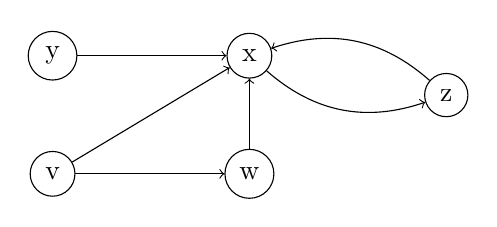
\begin{tikzpicture}
    \node[shape=circle,draw=black] (x) at (0,0) {x};
    \node[shape=circle,draw=black] (y) at (-2.5,0) {y};
    \node[shape=circle,draw=black] (z) at (2.5,-0.5) {z};
    \node[shape=circle,draw=black] (v) at (-2.5,-1.5) {v};
    \node[shape=circle,draw=black] (w) at (0,-1.5){w};
    

    \path [->] (v) edge node[left] {} (w);
    \path [->](v) edge node[left] {} (x);
    \path [->](w) edge node[left] {} (x);
    \path [->](x) edge[bend right=30] node[left] {} (z);
    \path [->](z) edge[bend right=30] node[right] {} (x);
    \path [->](y) edge node[left] {} (x);

 \end{tikzpicture}
    \end{center}
  \item Der gleiche Graph sieht ungerichtet wie folgt aus:
	          \begin{center}
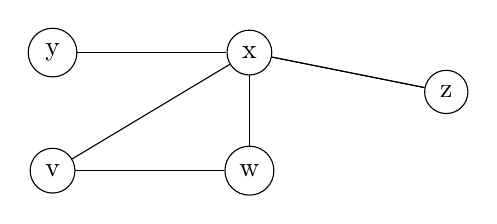
\begin{tikzpicture}
    \node[shape=circle,draw=black] (x) at (0,0) {x};
    \node[shape=circle,draw=black] (y) at (-2.5,0) {y};
    \node[shape=circle,draw=black] (z) at (2.5,-0.5) {z};
    \node[shape=circle,draw=black] (v) at (-2.5,-1.5) {v};
    \node[shape=circle,draw=black] (w) at (0,-1.5){w};


    \path [-] (v) edge node {} (w);
    \path [-](v) edge node {} (x);
    \path [-](w) edge node {} (x);
    \path [-](x) edge node {} (z);
    \path [-](z) edge node {} (x);
    \path [-](y) edge node {} (x);

 \end{tikzpicture}
    \end{center}
Wir bemerken insbesondere, dass $\{v,w\}=\{w,v\}$ im ungerichteten Graphen ist.
\end{itemize}
\end{example}
\begin{remark}
In Digraphen werden manchmal auch Kanten der Form $\{v,v\}, v \in V$ zugelassen.
\end{remark}
\begin{definition}
Sei $G=(V,E)$ ein Graph. Ein \emph{Weg} oder \emph{Pfad} von $v=v_0$ nach $w=v_r$ in $G$ ist eine Kantenfolge
\[
\pi=v_0,v_1,\ldots,v_r
\]
mit $r\ge1$ und
\begin{itemize}
	\item $(v_i, v_{i+1}) \in  E, i=0,\ldots,r-1$im Falle von Digraphen.
	\item $\{v_i,v_{i+1}\}\in E, i=0,\ldots,r-1$ im Falle von ungerichteten Graphen.
\end{itemize}
Der Weg heißt \emph{einfach}, falls
\begin{itemize}
	\item $v_0,\ldots,v_r$ paarweise verschieden sind oder
	\item $v_0,\ldots,v_r$  paarweise verschieden mit $v_0=v_r$.
\end{itemize}
Die \emph{Länge} von $\pi$ ist gegeben als $|\pi|=r$, ist also die Anzahl Knoten, die in $\pi$ durchlaufen werden.
Ein Knoten $w$ heißt von Knoten $v$ \emph{erreichbar}, falls ein Weg von $v$ nach $w$ existiert.
\end{definition}
\begin{example}
Bezogen auf Beispiel \ref{eg:graph1} ist:
\begin{itemize}
	\item $\pi_1= v,w$ ein einfacher Weg der Länge 1
	\item $\pi_2 =v,w,x$ ein einfacher Weg der Länge 2
	\item $\pi_3=v,w,x,z,x,z$ ein Weg der Länge 5
\end{itemize}
Im ungerichteten Fall ist 
\begin{itemize}
	\item $\pi_4=v,w,x,v$ ein einfacher Weg der Länge 3.
\end{itemize}
In beiden Fällen ist $z$ von $v$ erreichbar, im ungerichteten Fall gilt dies auch umgekehrt. Im gerichteten Fall ist v nicht von z erreichbar.
\end{example}
\begin{definition}
	\label{def:extendedgraph}
Sei $G=(V,E)$ ein Digraph und $v \in V$. Wir definieren:
\begin{itemize}
	\item die Menge der (direkten) \emph{Nachfahren} von v:
		\[
	post(v)=\{w \in V | (v,w) \in E\} 
		\]
	\item die Menge der (direkten) \emph{Vorfahren} von v:
		\[
		pre(v) = \{w \in  V | v \in  post(w)\} 
		\]
	\item die Menge der \emph{erreichbaren Knoten} von v:
		\[
		post^*(v)=\{w \in V | \text{ es gib einen Weg von v nach w}\} 
		\]
	\item die Menge aller Knoten die v erreichen können:
		\[
		pre^*(v)= \{w \in  V | v \in  post^*(w) \} 
		\]
	\item die Nachbarn als die Menge $post(v) \cup pre(v)$ von v
	\item und den Knotengrad $deg(v)$, welcher der Anzahl seiner Kanten entspricht.
\end{itemize}
\end{definition}
\begin{remark}
Mit den offensichtlichen Modifikationen kann die Definition \ref{def:extendedgraph} auch auf ungerichtete Graphen angewendet werden. Wir erhalten in diesem Fall für $v \in V$, dass
\begin{align*}
	post(v)&=pre(v) \\
	post^*(v) &= pre^*(v)
\end{align*}
\end{remark}
\begin{example}
Für den Digraphen aus Beispiel \ref{eg:graph1} gilt:
\begin{itemize}
	\item $post(v) = \{w,x\}$
	\item $post^*(v) = \{w,x,z\}$
	\item $pre(v)= \emptyset$
	\item $pre^*(v)= \emptyset$
	\item $deg(v)=2$
\end{itemize}
Für den ungerichteten Graphen gilt geändert:
\begin{itemize}
	\item $pre(v)=\{w,x\}$
	\item $pre^*(v)=\{w,x,y,z\}$
	\item $post^* = \{w,x,y,z\}$
\end{itemize}
\end{example}
